\section{Extending the methodology in the context of \gls{WCA}}

\todo[inline]{%
    Why do we need to extend the methodology? What was wrong with the approach in the previous section?
}

\subsection{Characterizing human behavior}

\cref{paper:olguinmunoz2021impact} describes a study designed to characterize the effects of system responsiveness on human behavior in step-based \gls{WCA}.
This corresponds to the first step in extending our EdgeDroid tool for the benchmarking of \gls{WCA}, first introduced in \cref{paper:olguinmunoz2018demoscaling,paper:olguinmunoz2019edgedroid}, with a more realistic model of human behavior.

We present in this paper the design and execution of a study in which undergraduate students of diverse fields of
study\footnote{%
    Participants were recruited from a pool of students enrolled in an undergraduate psychology course at \gls{CMU}.
}, were asked to interact with and follow the instructions given to them by a \gls{WCA} application.
Unbeknownst to the participants, the system responsiveness of the \gls{WCA} system was systematically altered in real time, and the resulting behavioral and physiological reactions were recorded.

With this study, we intended to answer four core research questions relating to human responses to decreased application responsiveness.
One, do subjects change the temporal profile of their actions in relation to system latency?
We expected this to be the case, although the extent or form of these changes were unknown.
Two, do users show signals of arousal in physiological responses to changes in system latency?
As latency increased and due to the added annoyance of dealing with a less responsive system, we expected users to begin showing signs of stress and frustration.
Three, are responses to delay effects in subjects mediated by cognition and/or emotion?
We expected delay effects in subjects to be mediated primarily by emotion, and in particular expected these effects to be correlated with the level of the reduction in system responsiveness.
And four, are these effects mediated by personality indicators in any way?
It was our hypothesis that, among others, the individual trait of \emph{neuroticism}~\cite{john1999big} would play a particularly important role in mediating effects of reduced system responsiveness on subjects.

\begin{figure}[tb]
    \centering
    \begin{subfigure}[t]{.49\textwidth}
        \centering
        \includegraphics[width=\textwidth]{publications/2021ImpactDelayedResponse/Fig4a}
        \caption{}\label{sfig:regularwcaexec}
    \end{subfigure}%
    \hfill%
    \begin{subfigure}[t]{.49\textwidth}
        \centering
        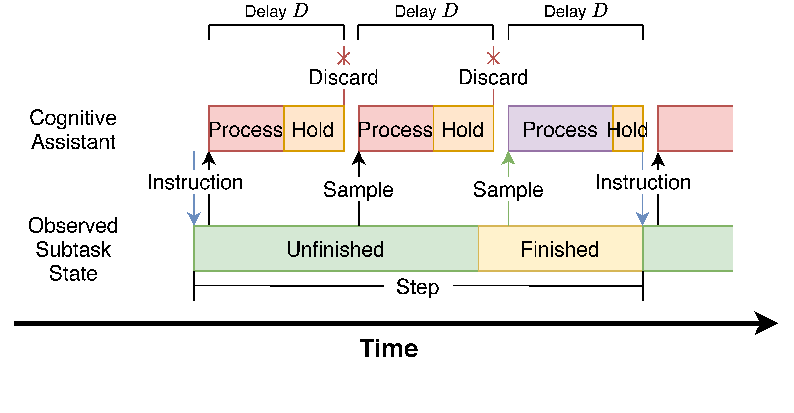
\includegraphics[width=\textwidth]{publications/2021ImpactDelayedResponse/Fig4b}
        \caption{}\label{sfig:delaywcaexec}
    \end{subfigure}
    \caption{%
        Comparison between normal task execution in the LEGO \gls{WCA}~\cite{chen2015early}~(\labelcref{sfig:regularwcaexec}) and modified task execution with delay in the experimental setup of \cref{paper:olguinmunoz2021impact}~(\labelcref{sfig:delaywcaexec}).
        In the experimental task, an additional variable segment of time is introduced immediately following the processing of the input frame in order to extend the perceived processing time of the input to a specific target interval of time denoted \emph{delay}.
    }\label{fig:regularwca-vs-delaywca}
\end{figure}

We employed a version of the step-based LEGO cognitive assistant first introduced by \citeauthor{chen2015early}~\cite{chen2015early}.
The software was modified to allow for the real-time alteration of system responsiveness by extending the processing interval of each input to a temporarily fixed value denoted \emph{delay}.
This is illustrated in \cref{fig:regularwca-vs-delaywca}.
If, during a series of steps, delay was set to a value \ensuremath{\mathbb{D}}, the feedback for each input frame was provided to the user exactly \ensuremath{\mathbb{D}} seconds after frame capture.
Furthermore, the assistant was instrumented to capture key application and task performance metrics in real time, in particular step execution time.
\todo[inline]{Task, latin square?}

In order to capture metrics relating to the emotional response of humans to changes in system responsiveness, participants were asked to wear an array of biometric sensors.
This array included devices to capture four physiological measures:
\begin{enumerate*}[itemjoin={{, }}, itemjoin*={{, and }}]
    \item \gls{GSR} (also known as electrodermal activity)
    \item accelerometer data from the dominant wrist
    \item brain activity in the form of \gls{EEG}
    \item heart rate
\end{enumerate*}.
Additionally, to measure individual differences in personality between them, participants were asked to complete two questionnaires previous to beginning the task, the \gls{BFI}~\cite{john1999big} and the \gls{ITQ}~\cite{witmer1998measuring}.



\todo[inline]{\cref{paper:olguinmunoz2021impact} describes the acquisition of the necessary data and insights for the
models.}

\todo[inline]{From introduction}

We intended to answer four core research questions relating to human responses to decreased application responsiveness.

\begin{itemize}
    \item \emph{Do subjects change the temporal profile of their actions in relation to system latency?}

    In line with previous research in this area, we expected subjects to change their temporal profiles as system
    \item responsiveness decreased.
    The extent or form of these changes were however unknown.
    We also hypothesized that large enough drops in responsiveness could lead to complete abandonment of the task by
    \item subjects.

    Our results show an emergent pacing effect on user actions as system responsiveness is reduced.
    While it would seem self-evident that users take longer to complete a task while using a system with low
    \item responsiveness --- as they have to wait longer for new instructions --- our study found that user slow-down
    \item represents a source of substantial additional delay.
    To be more precise, the data indicate that users slow down not only because they have to wait for the system to
    \item catch up, but that their reactions to new instructions is also delayed.
    Moreover, this effect scales with the decrease in responsiveness and remains for a while, even after system
    \item responsiveness improves.

    \item \emph{Do subjects show signals of arousal in physiological responses to changes in system latency?}

    We hypothesized subjects would show signs of stress and frustration as system latency increased, due to the added
    \item annoyance of dealing with an unresponsive system.

    The results we present, however, seem to refute this hypothesis.
    We were not able to detect any significant effects on the physiological signals obtained from the biometric
    \item sensors as system responsiveness was altered.

    \item \emph{Are responses to delay effects in subjects mediated by cognition and/or emotion?}

    In line with previous items, we expected delay effects in subjects to be mediated primarily by emotion.
    In particular, we expected emotional effects to be correlated with the strength of the added delay.

    The results point in a different direction though, indicating that reduced responsiveness in WCA systems leads to
    \item a disruption of participants' cognitive plan for the task and not to an emotional response.
    This is evidenced by the previously discussed pacing effect and the lack of significant physiological responses.

    \item \emph{Are these effects mediated by personality indicators in any way?}

    Finally, we hypothesized that the individual trait of \emph{neuroticism}~\cite{john1999:bfi} would play a role in
    \item mediating these effects, as it has previously been connected to intolerance for time
    \item delay~\cite{hirsh2008delay}.
    We also expected \emph{focus} and \emph{involvement}~\cite{witmer1998:itq} to play roles in this.

    The results obtained agree with our hypothesis.
    We found significant effects of neuroticism on the responses exhibited by subjects, and all three traits were
    \item found to play a role through factor analysis.

\end{itemize}

% Our results indicate that reduced responsiveness in WCA systems leads to a disruption of participants' cognitive
% plan for the task.
% This is evidenced by an emergent pacing effect on user actions as system responsiveness is reduced.
% While it would seem self-evident that users take longer to complete a task while using a system with low
% responsiveness --- as they have to wait longer for new instructions --- our study found that user slow-down
% represents a source of substantial additional delay.
% To be more precise, the data indicate that users slow down not only because they have to wait for the system to
% catch up, but that their reactions to new instructions is also delayed.
% Furthermore, this effect persists for a while after system response improves and is modulated by intrinsic
% personality traits, in particular, \emph{neuroticism}~\cite{john1999:bfi}.

We believe that these results provide concrete and relevant implications for WCA design, deployment, and optimization.
One example is the behavioral slow-down, as it extends application runtime significantly, and thus has clear and
direct implications for resource and power consumption.
Another is the fact that the adverse effects of delay on users do not immediately subside as delay is diminished ---
this has potential consequences for resource allocation strategies.
Moreover, in multi-user scenarios, the dependency of user slow-down effects on delay mean efficient resource
allocation across applications potentially looks different from what could be considered ``fair''.

Our hope is that the results we provide might prove useful for the understanding and optimization of deployments of
WCA.\@
These results represent unexpected, valuable findings, which can be employed to model and understand how users
interact with latency in applications and systems, and develop resource allocation and power optimization strategies.
Additionally, we hope that the results we provide might pave the way for the improvement of performance evaluation
tools such as our previous work in \cite{olguin:2018, olguin:2019}.
Such systems would greatly benefit from this knowledge, as it would allow for the design and implementation of
realistic models of human behavior, making highly accurate benchmarks a reality in the domain of WCA.\@

\todo[inline]{From discussion}

We start our discussion with the main results of our experimentation presented in the previous section:

\begin{itemize}
    \item Firstly, and perhaps most importantly, we find that a system slow-down induces an \textit{additional}
    \item behavioral slow-down.
    That is, as system responsiveness decreases, our data indicates that users significantly slow-down in their
    \item execution of the task.
    This slow-down scales with the decrease in responsiveness; compared to the no-delay case, participants were on
    \item average \SI{12}{\percent} slower at \SI{1.65}{\second} delay and \SI{26}{\percent} at \SI{3.0}{\second} delay.
    Moreover, there is a temporal component to this effect; users become progressively slower the more time passes
    \item with reduced system responsiveness.

    \item Secondly, we find that the effects of behavioral slow-down due to impaired system responsiveness
    \item \emph{remain} for at least a few steps after system responsiveness improves.
    This is evidenced by the longer per-step-execution times of the first four steps of blocks immediately following
    \item a high-delay block, as pictured in \cref{fig:exectime:transition}.
    The question of whether any lingering effect can be measured after these four steps remains open.

    \item Thirdly, we evidence a speed-up in execution time over a series of steps; that is, subjects get faster at
    \item performing steps as the task progresses.
    However, the strength of this effect decreases as delay increases.
    Whereas for blocks without delay users performed the last four steps of a 12-step block on average
    \item \SI{36}{\percent} faster than the first four, at the maximum delay this effect practically disappears.

    \item Fourthly, in terms of inter-subject differences, PCA revealed three main factors governing users' response
    \item to delay.
    The first factor represents sensitivity to delay as moderated by the ``Big Five'' personality trait of
    \item neuroticism and both measures of immersion: focus and involvement.
    Factor two and three represent dedication to the task as opposed to delay intolerance and reflect variables
    \item related to attentiveness, respectively.
    In simple terms, these results suggest that the effects of delay are most potent in individuals who are sensitive
    \item and involved in the task.
    The findings appear selective to cognitive assistance tasks like the present ones, inasmuch as the same measures
    \item did not correlate with outcomes in other computer-intensive environments such as immersive
    \item VR~\cite{quesnel2018you}.
    These correlations are also consistent with previous findings indicating that individuals scoring high in
    \item neuroticism tend to be intolerant to delayed reward~\cite{hirsh2008delay}.
\end{itemize}

A central question therefore arises: to which physio- and psychological mechanisms can these findings, most
importantly the substantial slow-down in task execution, be attributed?

In \cref{sec:background}, we initially considered the possibility that delays might produce negative emotional
reactions.
These could in turn elicit generalized arousal.
We also postulated that adapting to delay might progressively deplete cognitive resources in users.
However, the present data provide relatively little support for these alternatives, in that the predicted measures
did not produce the expected statistical trends.
Specifically, physiological measures of GSR and HR failed to show evidence of differential arousal under long vs.\
short delays, and speed-induced errors and non-completions predicted by resource depletion were not observed.
The acceleration data further did not indicate that extended delay significantly increases erratic movement.
% physiological measures of GSR and HR failed to show evidence of differential arousal under long vs.\ short delays,
% and speed-induced errors and non-completions predicted by resource depletion were not observed.
% The acceleration data further do not indicate that extended delay increases erratic movement.
To the contrary, the data suggest this effect results from a delay in movement after an instruction is introduced.
That is, users fail to capitalize on the new information as quickly as they could.
Thus, contrary to our preliminary postulations, behavioral effects seem to arise from impaired cognitive control
mechanisms, and not from emotion or resource depletion.
We hypothesize that the effects of feedback latency can best be understood as changes in the use of a cognitive plan.
As was described in \cref{sec:experimentaldesign,fig:lego:hierarchical}, complex cognitive and motor tasks have been
modeled as the unfolding of a hierarchy of command, from high-level plans to physical output.
Long system latencies, we propose, disrupt the automating of such a plan, instead relegating it to attention-based
control at the step-by-step level that is easily diverted.
This also provides a possible explanation for the lingering effects of delay after an acceptable system
responsiveness is restored, as users needs time re-adjust and re-automate their cognitive plans.

As to the applicability of our findings to other applications, it must be noted that these results pertain to a
specific class of applications, namely step-based task-guidance WCA.\@
However, we would expect our findings to extend to similar applications, as long as they follow the same pattern of
seamless interaction --- i.e.\ such that the user does not need explicitly interact with the application to advance
the state.

The results here presented provide a number of possible implications for WCA system design and optimization, both for
single and multi-application flows.

\begin{itemize}

    \item Due to the behavioral slow-down in users, even short-term reductions in responsiveness will lead to
    \item significantly extended application lifetimes.
    This has direct implications for resource and power consumption.

    \item The fact that the adverse effects of delay on users do not immediately disappear as the system returns to a
    \item high-responsive state could have unconventional consequences for resource allocation.
    This is of particular importance, for instance, for cases where the user may be able to finish the task before
    \item these effects subside.
    In such cases, the limited potential gains might not justify diverting valuable system resources to the impaired
    \item application.

    \item In multi-user environments, the time dependency of user slow-down effects mean that fair degradation of
    \item system responsiveness across applications may not ultimately be beneficial to the system as a whole.
    Take for instance two applications on the same system which negatively interfere with each other.
    The longer they interfere with each other, the longer their respective lifetimes are going to be, which in turn
    \item causes them to interfere even longer, potentially entering a positive feedback loop.
    In such a case, prioritizing one over the other rather than trying to improve responsiveness for both might lead
    \item to resources being freed up faster system-wide.

    \item Based on our findings relating individual differences between users and their sensitivity to delays, it
    \item might also be possible to extrapolate user characteristics from measured execution times.
    This could prove a valuable tool for load balancing, for instance by prioritizing resource allocation to users
    \item with a higher sensitivity to system-state degradation.
    However, this remains an open challenge.

\end{itemize}

To wrap up, we believe the present data provide novel and unexpected insights for the understanding and optimizing of
WCA deployments.
Although more subtle than expected, and in some cases somewhat counterintuitive, these insights represent a valuable
tool to tackle inefficiencies in these systems.
Moreover, we also argue these findings represent a first step towards a full-fledged understanding of the
relationship between application responsiveness and human behavior.
More research in this area will surely uncover more complex and interesting behaviors.
Finally, we believe the data provide parameters that can usefully be integrated into cognitive models of WCA that
might be constructed under existing architectures like ACT-R.
These same parameters could be used to modulate the timing and generation of inputs in trace-based workload
generation tools such as the EdgeDroid platform~\cite{olguin:2018,olguin:2019}, allowing the tool to use the same
trace to generate workloads for a multitude of different user profiles.

\todo[inline]{Some diagrams, plots, and results}

\begin{figure}[h]
    \centering
    \begin{subfigure}[t]{.49\textwidth}
        \centering
        \includegraphics[width=\textwidth]{publications/2021ImpactDelayedResponse/Fig4a.eps}
        \caption{Structure of a step in a generic cognitive assistance application.
        The assistant provides an instruction to the user and continuously samples the step state; inputs captured
        while the step is unfinished are silently ``discarded'' (i.e.\ they do not cause the generation of a new
        instruction).
        % by the assistant, as they do not contain relevant information.
        Once the user finishes performing the step, the next sample \emph{will} cause the generation of a new
        instruction.
        % which will subsequently be provided to the user.}%
        }
        \label{fig:cogassist:step}
    \end{subfigure}%
    % \medskip%
    \hfill%
    \begin{subfigure}[t]{.49\textwidth}
        \centering
        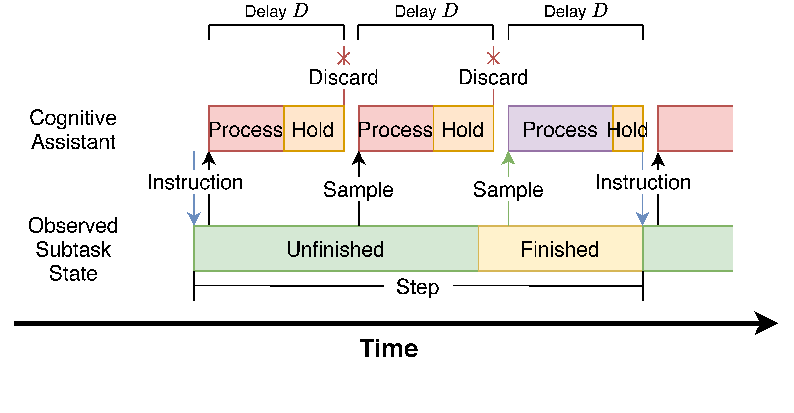
\includegraphics[width=\textwidth]{publications/2021ImpactDelayedResponse/Fig4b.eps}
        \caption{In the experimental task, an additional variable segment of time is introduced immediately following
        the processing of the input frame in order to extend the perceived processing time of the input to a specific
        target delay.}%
        \label{fig:cogassist:step:delay}
    \end{subfigure}
    \medskip%
    \begin{subfigure}[t]{.49\textwidth}
        \centering
        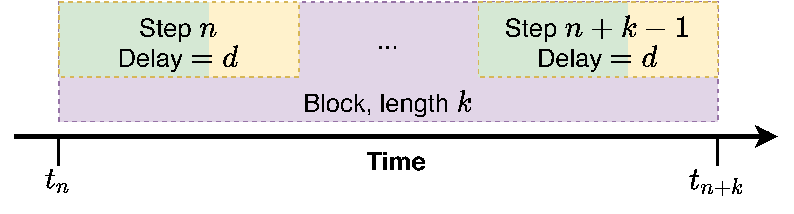
\includegraphics[width=\textwidth]{publications/2021ImpactDelayedResponse/Fig4c.eps}
        \caption{Structure of a block in the experimental task.}%
        \label{fig:cogassist:block}
    \end{subfigure}%
    % \medskip%
    \hfill%
    \begin{subfigure}[t]{.49\textwidth}
        \centering
        \includegraphics[width=\textwidth]{publications/2021ImpactDelayedResponse/Fig4d.eps}
        \caption{Visualization of the execution time of a step.}%
        \label{fig:exectime:diagram}
    \end{subfigure}%
    % \medskip%
    \caption{Components of the cognitive assistance task.}
\end{figure}

\begin{figure}[h]
    \centering
    \includegraphics[width=.8\textwidth]{publications/2021ImpactDelayedResponse/Fig6.eps}
    \caption{Per-step execution time by block length vs.\ delay. Error bars indicate the Standard Error of the Mean
        (S.E.M.)}\label{fig:exectime}%
\end{figure}

\begin{figure}[h]
    \centering
    \includegraphics[width=.8\textwidth]{publications/2021ImpactDelayedResponse/Fig7.eps}
    \caption{Mean per-step execution time vs.\ delay, by step slice.
    Error bars indicate S.E.M.}
    \label{fig:exectime:delay:slice}
\end{figure}

\begin{figure}[h]
    \centering
    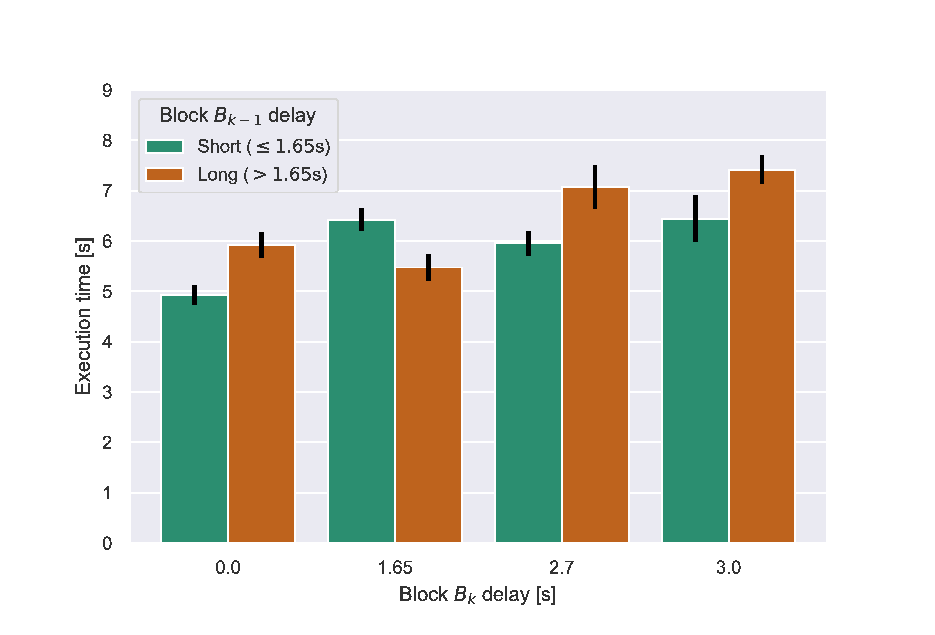
\includegraphics[width=.8\textwidth]{publications/2021ImpactDelayedResponse/Fig8.eps}
    \caption{Per-step execution time across the first four steps after a block transition from block \( B_{k-1} \) to
        \( B_k \). Error bars indicate S.E.M.}\label{fig:exectime:transition}%
\end{figure}

\begin{table}[h]
    \centering
    \caption{Principal Component Analysis}\label{tab:pca}
    \begin{subtable}[h]{\textwidth}
        \centering
        \caption{Main components identified.}
        \setlength{\tabcolsep}{0pt} % let TeX compute the intercolumn space
        \begin{tabular*}{\textwidth}{@{\extracolsep{\fill}\quad}lrrr@{}}
            \toprule
            \textbf{Factor} & \textbf{Comp. 1} & \textbf{Comp. 2}
            & \textbf{Comp. 3} \\
            \midrule
            BFI Conscientiousness & \textcolor{lightgray}{\( -0.022 \)} & \( 0.668 \)
            & \textcolor{lightgray}{\( -0.481 \)} \\
            BFI Neuroticism & \( 0.600 \) & \( -0.678 \)
            & \textcolor{lightgray}{\( -0.118 \)} \\
            ITQ Focus & \( 0.678 \) &
            \textcolor{lightgray}{\( 0.203 \)} & \( 0.504 \) \\
            ITQ Involvement & \( 0.573 \) & \( 0.540 \)
            & \textcolor{lightgray}{\( 0.417 \)} \\
            Exec. Time (delay 3.0 s, length 12) & \( 0.758 \) &
            \textcolor{lightgray}{\( -0.178 \)}
            & \textcolor{lightgray}{\( -0.348 \)}
            \\
            Log EEG power \( \alpha + \beta \) Slice 1 & \textcolor{lightgray}{\( -0.436 \)} &
            \textcolor{lightgray}{\( -0.251 \)}
            & \( 0.589 \)
            \\
            \bottomrule
        \end{tabular*}
    \end{subtable}
    \newline
    \medskip
    \newline
    \begin{subtable}[h]{\textwidth}
        \centering
        \caption{Percentages of variance explained by the components.}
        \begin{tabular*}{\textwidth}{@{\extracolsep{\fill}\quad}lrrrr@{}}
            \toprule
            {} & \textbf{Comp. 1} & \textbf{Comp. 2} & \textbf{Comp. 3} & \textbf{Total}
            \\
            \midrule
            Explained Variance & \SI{31.88}{\percent} & \SI{22.22}{\percent} & \SI{19.03}{\percent}
            & \SI{73.13}{\percent}
            \\
            \bottomrule
        \end{tabular*}
    \end{subtable}
\end{table}

\subsection{Emulating human behavior}

We introduce the first, to our knowledge, data-driven model for human timings in \gls{WCA} applications.
Using the data collected for \textcite{olguinmunoz:impact2021} as a base, we build a stochastic model which takes as
input past measurements of system responsiveness and produces realistic step execution times.
We also introduce a novel way to generate dynamic traces of frames for \gls{WCA} applications which can be combined
with the timing model for a full end-to-end emulation of a human.
We name this new model \emph{EdgeDroid 2.0}; a direct, more realistic evolution of our initial EdgeDroid
approach~\cite{olguin2018scaling,olguin2019edgedroid}.

The study and benchmarking of \gls{WCA} applications is a challenging discipline due to these application's intrinsic
human-in-the-loop nature.
Humans are notoriously unreliable, and greatly complicate the scalability and repeatability of experiments.
Furthermore, recruiting large enough cohorts of humans for large-scale experimentation is both greatly time-consuming
and prohibitively expensive for many research groups.

In the first half of this paper, we have introduced the EdgeDroid 2.0 model of human timing behavior for \gls{WCA},
the first data-driven model for human timings in \gls{WCA} applications.
This model represents a stochastic approach to execution time modeling which builds upon the data collected for
\textcite{olguinmunoz:impact2021}.
Together with this model, we have also introduced a novel procedure for the generation of synthetic traces of frames in step-based \gls{WCA}, allowing for a full end-to-end emulation of a human when combined with the timing model.

\todo[inline]{TODO: Some relevant results. Need to add paper to thesis.}